\documentclass[letterpaper,10pt]{article}
\usepackage[final]{pgtest}
\usepackage[T1]{fontenc}
\usepackage{lmodern}
\usepackage{amsmath,amssymb,amsthm}
\usepackage{graphicx}
\usepackage{booktabs}
\usepackage[hidelinks]{hyperref}
\hypersetup{pdftitle={Gated Diffusion Planning for Safe Navigation},
  pdfauthor={Ada Lovelace, Alan Turing, Grace Hopper}}

\newtheorem{theorem}{Theorem}
\newtheorem{lemma}{Lemma}
\newtheorem{assumption}{Assumption}
\newtheorem{definition}{Definition}

\title{Gated Diffusion Planning for Safe Navigation}
\author{Ada Lovelace\\Analytical Engine Lab\\\texttt{ada@test.edu}
  \and Alan Turing\\Computable Numbers Inst.\\\texttt{alan@icn.org}
  \and Grace Hopper\\Compiler Research Center\\\texttt{grace@crc.org}}

\begin{document}
\maketitle

\begin{abstract}
Sampling-based planners are fast but offer no safety certificate for the plans they return.
We present a gated diffusion planner that accepts a sampled plan only when a reachability test
certifies it. On a cluttered navigation benchmark the planner reaches a success rate of
85.7\% and reduces collisions by 40\% relative to the strongest baseline.
\end{abstract}

\section{Introduction}\label{sec:intro}
Diffusion models generate diverse plans for robot navigation, but a sampled plan may still
collide with an obstacle. Classical model predictive control (MPC) handles constraints
explicitly, yet it needs a good initial guess. We combine the two: a gated diffusion planner
(GDP) samples candidate plans and an MPC layer repairs them, and a reachability gate accepts
a plan only if it is certified safe.

Our contributions are:
\begin{itemize}
  \item a gate that certifies sampled plans with high probability (Theorem~\ref{thm:main});
  \item an evaluation on a cluttered navigation benchmark (Section~\ref{sec:exp}).
\end{itemize}

\section{Preliminaries}\label{sec:prelim}
Let $x_t \in \mathbb{R}^n$ denote the robot state at time $t$ and let $\mathcal{X}$ denote the
safe set. The dynamics are $x_{t+1} = f(x_t, u_t) + w_t$, where $w_t$ is the process noise.

\begin{assumption}\label{asm:lip}
The map $f$ is $L$-Lipschitz in its first argument.
\end{assumption}

\begin{assumption}\label{asm:noise}
The noise satisfies $\|w_t\| \le \sigma$ for all $t$.
\end{assumption}

\section{Method}\label{sec:method}
The planner draws $N$ candidate plans from a diffusion model~\cite{ho2020denoising} and passes
each through the gate. The gate follows the scenario approach~\cite{campi2008exact}, and the
MPC layer follows standard practice~\cite{rawlings2017model}.

\begin{theorem}\label{thm:main}
Under Assumptions~\ref{asm:lip} and~\ref{asm:noise}, every plan accepted by the gate stays in
$\mathcal{X}$ with probability at least $1-\delta$.
\end{theorem}

\begin{proof}
By Assumption~\ref{asm:lip}, the deviation of two trajectories grows by at most a factor $L$
per step. By Assumption~\ref{asm:noise}, each step adds at most $\sigma$. The scenario bound
then gives the probability $1-\delta$.
\end{proof}


\section{Experiments}\label{sec:exp}
We compare GDP with an MPC baseline on 200 navigation episodes (setup in Section~\ref{sec:setup}). Table~\ref{tab:main} reports
the success rate and the number of collisions per 100 episodes, and Figure~\ref{fig:plot}
shows the success rate as the noise level grows.

\begin{table}[t]
  \centering
  \caption{Results on the cluttered navigation benchmark.}\label{tab:main}
  \begin{tabular}{lcc}
    \toprule
    Method & Success (\%) & Collisions \\
    \midrule
    MPC baseline & 71.2 & 5.0 \\
    GDP (ours) & 85.7 & 3.0 \\
    \bottomrule
  \end{tabular}
\end{table}

\begin{figure}[t]
  \centering
  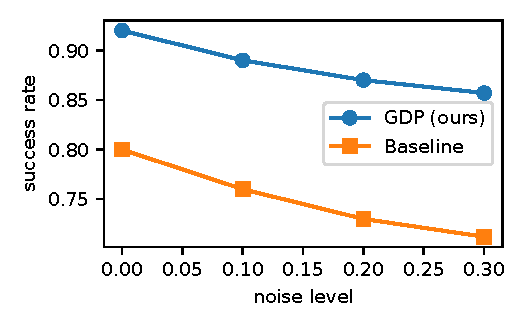
\includegraphics[width=0.6\linewidth]{fig/plot.pdf}
  \caption{Success rate of GDP and the MPC baseline as the noise level grows.}\label{fig:plot}
\end{figure}

\section{Limitations}\label{sec:limits}
The certificate of Theorem~\ref{thm:main} holds only under the Lipschitz and bounded-noise
assumptions; real sensors can violate the noise bound during fast motion. The gate rejects
plans conservatively, so in narrow corridors the planner may fail to return any plan within
the time budget. Our evaluation uses a single simulated benchmark, and we have not yet tested
the planner on hardware, where unmodelled delays could break the guarantee.

\section{Conclusion}\label{sec:conclusion}
GDP certifies sampled plans and reaches a success rate of 85.7\% on the benchmark while
reducing collisions by 40\%.

\acknowledgments{We thank the anonymous reviewers. This work was supported by grant GRANT-12345.}

\bibliographystyle{plain}
\bibliography{refs}

\appendix
\section{Restated result}\label{sec:appendix}
\begin{theorem}[Restatement of Theorem~\ref{thm:main}]
Under Assumptions~\ref{asm:lip} and~\ref{asm:noise}, every plan accepted by the gate stays in
$\mathcal{X}$ with probability at least $1-\delta$.
\end{theorem}

\end{document}
